\let\negmedspace\undefined
\let\negthickspace\undefined
\documentclass[journal,12pt,onecolumn]{IEEEtran}
\usepackage{cite}
\usepackage{amsmath,amssymb,amsfonts,amsthm}
\usepackage{algorithmic}
\usepackage{graphicx}
\graphicspath{{./figs/}}
\usepackage{textcomp}
\usepackage{xcolor}
\usepackage{txfonts}
\usepackage{listings}
\usepackage{enumitem}
\usepackage{mathtools}
\usepackage{gensymb}
\usepackage{comment}
\usepackage{caption}
\usepackage[breaklinks=true]{hyperref}
\usepackage{tkz-euclide} 
\usepackage{listings}
\usepackage{gvv}                                        
%\def\inputGnumericTable{}                                 
\usepackage[latin1]{inputenc}     
\usepackage{xparse}
\usepackage{color}                                            
\usepackage{array}                                            
\usepackage{longtable}                                       
\usepackage{calc}                                             
\usepackage{multirow}
\usepackage{multicol}
\usepackage{hhline}                                           
\usepackage{ifthen}                                           
\usepackage{lscape}
\usepackage{tabularx}
\usepackage{array}
\usepackage{float}
\newtheorem{theorem}{Theorem}[section]
\newtheorem{problem}{Problem}
\newtheorem{proposition}{Proposition}[section]
\newtheorem{lemma}{Lemma}[section]
\newtheorem{corollary}[theorem]{Corollary}
\newtheorem{example}{Example}[section]
\newtheorem{definition}[problem]{Definition}
\newcommand{\BEQA}{\begin{eqnarray}}
\newcommand{\EEQA}{\end{eqnarray}}
\newcommand{\define}{\stackrel{\triangle}{=}}
\theoremstyle{remark}
\newtheorem{rem}{Remark}



\title{\LARGE \textbf{AE - 2013}}
\author{\Large EE25BTECH11048 - Revanth Siva Kumar.D}
\date{}

\begin{document}

\maketitle
\begin{flushleft}
\begin{enumerate}


\item 
For a flow through a Prandtl-Meyer expansion wave 
\hfill(GATE AE 2009)
\begin{multicols}{2}
\begin{enumerate}
\item Mach number stays constant.
\item Entropy stays constant.
\item Temperature stays constant.
\item Density stays constant.
\end{enumerate}
\end{multicols}

\item 
For two-dimensional irrotational and incompressible flows
\hfill(GATE AE 2009)
\begin{multicols}{2}
\begin{enumerate}
\item Both potential and stream functions satisfy the Laplace equation.
\item Potential function must satisfy the Laplace equation but the stream function need not.
\item Stream function must satisfy the Laplace equation but the potential function need not.
\item Neither the stream function nor the potential function need to satisfy the Laplace equation.
\end{enumerate}
\end{multicols}

\item 
A trailing edge plain flap deflected downward increases the lift coefficient of an airfoil by
\hfill(GATE AE 2009)
\begin{enumerate}
\item Increasing the effective camber of the airfoil.
\item Delaying the separation of the flow from the airfoil surface.
\item Increasing the local airspeed near the trailing edge.
\item Controlling the growth of the boundary layer thickness along the airfoil surface.
\end{enumerate}

\item 
Thin airfoil theory predicts that the lift slope 
\[
\frac{dc_l}{d\alpha} = 2\pi
\]
for
\hfill(GATE AE 2009)
\begin{multicols}{2}
\begin{enumerate}
\item Symmetric airfoils only.
\item Cambered airfoils only.
\item Any airfoil shape.
\item Joukowski airfoils only.
\end{enumerate}
\end{multicols}

\item 
The ordinary differential equation 
\[
\frac{d^2 y}{dx^2} + ky = 0
\]
where \(k\) is real and positive
\hfill(GATE AE 2009)

\begin{enumerate}
\item is non-linear
\item has a characteristic equation with one real and one complex root
\item has a characteristic equation with two real roots
\item has a complementary function that is simple harmonic
\end{enumerate}


\item 
A non-trivial solution to the \( (n \times n) \) system of equations 
\[
[A]\{x\} = \{0\}
\]
where \( \{0\} \) is the null vector
\hfill(GATE AE 2009)
\begin{enumerate}
\item can never be found
\item may be found only if \([A]\) is not singular
\item may be found only if \([A]\) is an orthogonal matrix
\item may be found only if \([A]\) has at least one eigenvalue equal to zero
\end{enumerate}
\item 
For a plane strain problem, the stresses satisfy the condition
\hfill(GATE AE 2009)
\begin{enumerate}
\item \(\tau_{xz} = \tau_{yz} = \sigma_z = 0\)
\item \(\tau_{xz} = \tau_{yz} = 0, \sigma_z = \nu (\sigma_x + \sigma_y)\)
\item \(\tau_{xz} = \tau_{yz} = 0, \sigma_z = \nu \tau_{xy}\)
\item \(\tau_{xz} = \tau_{yz} = 0, \sigma_z = \nu (\sigma_x + \sigma_y) + (1 - \nu)\tau_{xy}\)
\end{enumerate}

\item 
The propulsive efficiency of a turbo-jet engine moving at velocity \(U_\infty\) and having exhaust velocity \(U_e\) with respect to the engine is given by
\hfill(GATE AE 2009)
\begin{multicols}{2}
\begin{enumerate}
\item \(\dfrac{2}{\dfrac{U_\infty}{U_e} + 1}\)
\item \(1 - \dfrac{U_\infty}{U_e}\)
\item \(\dfrac{2U_\infty U_e}{U_e^2 + U_\infty^2}\)
\item \(\dfrac{2U_\infty}{U_e + U_\infty}\)
\end{enumerate}
\end{multicols}

\item 
An aircraft is flying at \(M = 2\) where the ambient temperature around the aircraft is \(250~K\). If the specific heat ratio for air \(\gamma = 1.4\), the stagnation temperature on the surface of the aircraft is
\hfill(GATE AE 2009)
\begin{multicols}{2}
\begin{enumerate}
\item 200 K
\item 450 K
\item 350 K
\item 1450 K
\end{enumerate}
\end{multicols}

\item 
The division of feed air to an aircraft gas-turbine combustor into primary and secondary streams serves which of the following purposes?  
P. a flammable mixture can be formed  
Q. cooling of combustor liner and flame tube can be accomplished  
R. specific fuel consumption can be reduced
\hfill(GATE AE 2009)
\begin{multicols}{2}
\begin{enumerate}
\item P and R
\item Q and R
\item P and Q
\item P, Q and R
\end{enumerate}
\end{multicols}

\item 
Classify the following propellants as: cryogenic (C), semi-cryogenic (SC), compressed gas (CG) and earth storable (ES)

\begin{itemize}
\item \( \mathrm{N_2O_4\text{-}UDMH} \): nitrogen tetra oxide and unsymmetrical di-methyl hydrazine  
\item \( \mathrm{LOX\text{-}RP1} \): liquid oxygen and kerosene  
\item \( \mathrm{LOX\text{-}LH_2} \): liquid oxygen and liquid hydrogen  
\item \( \mathrm{N_2} \): nitrogen gas  
\end{itemize}
\hfill(GATE AE 2009)
\begin{multicols}{2}
\begin{enumerate}
\item \( \mathrm{N_2O_4\text{-}UDMH} \) (ES), \( \mathrm{LOX\text{-}RP1} \) (C), \( \mathrm{LOX\text{-}LH_2} \) (C), \( \mathrm{N_2} \) (C)
\item \( \mathrm{N_2O_4\text{-}UDMH} \) (SC), \( \mathrm{LOX\text{-}RP1} \) (SC), \( \mathrm{LOX\text{-}LH_2} \) (C), \( \mathrm{N_2} \) (C)
\item \( \mathrm{N_2O_4\text{-}UDMH} \) (ES), \( \mathrm{LOX\text{-}RP1} \) (SC), \( \mathrm{LOX\text{-}LH_2} \) (C), \( \mathrm{N_2} \) (CG)
\item \( \mathrm{N_2O_4\text{-}UDMH} \) (ES), \( \mathrm{LOX\text{-}RP1} \) (C), \( \mathrm{LOX\text{-}LH_2} \) (C), \( \mathrm{N_2} \) (CG)
\end{enumerate}
\end{multicols}

\item 
A conventional altimeter is a
\hfill(GATE AE 2009)
\begin{multicols}{2}
\begin{enumerate}
\item Pressure transducer
\item Temperature transducer
\item Density transducer
\item Velocity transducer
\end{enumerate}
\end{multicols}

\item 
The relation between an airplane's true airspeed \(V_{TAS}\) and equivalent airspeed \(V_{EAS}\) in terms of the density ratio \(\sigma = \dfrac{\rho}{\rho_0}\), where \(\rho_0\) is the air density at sea-level and \(\rho\) is the air density at the altitude at which the airplane is flying, is given by the formula:
\hfill(GATE AE 2009)
\begin{multicols}{2}
\begin{enumerate}
\item \(\dfrac{V_{EAS}}{V_{TAS}} = \sigma\)
\item \(\dfrac{V_{EAS}}{V_{TAS}} = \sigma^2\)
\item \(\dfrac{V_{EAS}}{V_{TAS}} = \sqrt{\sigma}\)
\item \(\dfrac{V_{EAS}}{V_{TAS}} = \dfrac{1}{\sqrt{\sigma}}\)
\end{enumerate}
\end{multicols}

\item 
An unswept fixed-winged aircraft has a large roll stability if the wing is placed
\hfill(GATE AE 2009)
\begin{multicols}{2}
\begin{enumerate}
\item low on the fuselage and has negative dihedral angle
\item low on the fuselage and has positive dihedral angle
\item high on the fuselage and has negative dihedral angle
\item high on the fuselage and has positive dihedral angle
\end{enumerate}
\end{multicols}

\item 
Thrust available from a turbojet engine
\hfill(GATE AE 2009)
\begin{multicols}{2}
\begin{enumerate}
\item increases as altitude increases
\item increases up to the tropopause and then decreases
\item remains constant at all altitudes
\item decreases as altitude increases
\end{enumerate}
\end{multicols}

\item 
If \(C_{m_{CG}}\) is the pitching moment coefficient about the center of gravity of an aircraft, and \(\alpha\) is the angle of attack, then
\[
\frac{dC_{m_{CG}}}{d\alpha}
\]
is
\hfill(GATE AE 2009)

\begin{enumerate}
\item a stability derivative which represents stiffness in pitch
\item a stability derivative which represents damping in pitch
\item a control derivative in pitch
\item positive for an aircraft that is stable in pitch
\end{enumerate}

\item 
The life of a geo-stationary communications satellite is limited by
\hfill(GATE AE 2009)

\begin{enumerate}
\item the working life of the on-board electronic circuitry
\item the time it takes for its orbit to decay due to atmospheric drag
\item the quantity of on-board fuel available for station-keeping
\item the number of meteorite impacts that the satellite structure can withstand before breaking up
\end{enumerate}

\item 
For a critically damped single degree of freedom spring-mass-damper system with a damping constant \(c\) of 4 Ns/m and spring constant \(k\) of 16 N/m, the system mass \(m\) is
\hfill(GATE AE 2009)
\begin{multicols}{2}
\begin{enumerate}
\item 0.5 kg
\item 0.25 kg
\item 2 kg
\item 4 kg
\end{enumerate}
\end{multicols}

\item 
In a thin walled rectangular tube subjected to equal and opposite forces \(P\) as shown in the figure, the shear stress along leg AB is  
\begin{figure}[H]
    \centering
    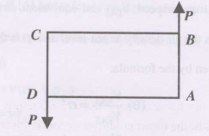
\includegraphics[width=0.5\columnwidth]{figs/19.png}
    \caption{}
    \label{fig:placeholder}
\end{figure}
\hfill(GATE AE 2009)
\begin{multicols}{2}
\begin{enumerate}
\item zero
\item constant non-zero
\item varies linearly
\item varies parabolically
\end{enumerate}
\end{multicols}

\item 
For the thin walled beam cross section as shown in the figure, the shear centre lies at  
\begin{figure}[H]
    \centering
    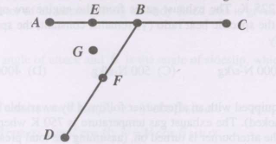
\includegraphics[width=0.5\columnwidth]{figs/20.png}
    \caption{}
    \label{fig:placeholder}
\end{figure}
\hfill(GATE AE 2009)
\begin{multicols}{2}
\begin{enumerate}
\item Mid point of AB, i.e. at point E
\item Mid point of BD, i.e. at point F
\item Junction point B
\item at a point G lying within the area ABC
\end{enumerate}
\end{multicols}

\item 
Let \( M_0 \) be the total mass of a single stage rocket, \( M_p \) be the total mass of propellant, \( M_L \) be the mass of payload carried by the rocket and \( M_S \) be the mass of inert structural components. If \( I_{sp} \) is the specific impulse of the propulsion system (in seconds) and \( g \) is the acceleration due to gravity, then the maximum velocity that can be attained by the rocket vehicle in the absence of gravity and atmospheric drag is given by
\[
g I_{sp} \ln \left( \frac{M_0}{M_p} \right)
\]

\hfill(GATE AE 2009)
\begin{multicols}{2}
\begin{enumerate}
\item \( g I_{sp} \ln \left( \frac{M_0}{M_p} \right) \)
\item \( g I_{sp} \ln \left( \frac{M_0}{M_L + M_S} - 1 \right) \)
\item \( g I_{sp} \ln \left( \frac{M_0}{M_S} \right) \)
\item \( g I_{sp} \ln \left( \frac{M_0}{M_0 - M_P} \right) \)
\end{enumerate}
\end{multicols}

\item 
An ideal axial compressor is driven by an ideal turbine across which the total temperature ratio is 0.667. If the total temperature at turbine inlet is \(T_0 = 1500~K\) and specific heat of gas \(c_p = 1~kJ/kg/K\), the power drawn by the compressor per unit mass flow rate of air is approximately

\hfill(GATE AE 2009)
\begin{multicols}{2}
\begin{enumerate}
\item 300 kW/kg/s
\item 1000 kW/kg/s
\item 600 kW/kg/s
\item 500 kW/kg/s
\end{enumerate}
\end{multicols}

\item 
The performance of a solid rocket motor is improved by replacing the old propellant with a new one. The new propellant gives a combustion temperature 40\% higher than the previous propellant without appreciable change in molecular weight of combustion products and other operating parameters. By approximately what percentage is the specific impulse of the new motor higher than the old one?

\hfill(GATE AE 2009)
\begin{multicols}{2}
\begin{enumerate}
\item 18\%
\item 96\%
\item 42\%
\item 112\%
\end{enumerate}
\end{multicols}

\item 
A solid rocket motor has an end burning grain of cross-sectional area \(A_{CS} = 0.4~m^2\). The density of propellant is \(\rho_p = 1500~kg/m^3\) and has linear regression rate \(\dot{r} = 5~mm/s\). If the specific impulse of the propulsion system is \(I_{sp} = 200~\text{seconds}\), the thrust produced by the motor is approximately

\hfill(GATE AE 2009)
\begin{multicols}{2}
\begin{enumerate}
\item 3 kN
\item 6 kN
\item 1.5 kN
\item 12 kN
\end{enumerate}
\end{multicols}

\item 
An ideal ramjet is flying at an altitude of 10 km with a velocity of 1 km/s. The ambient pressure is \(0.25~\text{bar}\) and temperature is \(225~\text{K}\). The exhaust gases from the engine are optimally expanded and leave the nozzle at \(900~\text{K}\). If the specific heat ratio \((\gamma)\) remains constant, the specific thrust developed by the engine is approximately  
\hfill(GATE AE 2009)
\begin{multicols}{2}
\begin{enumerate}
\item 1000 N-s/kg
\item 2000 N-s/kg
\item 500 N-s/kg
\item 4000 N-s/kg
\end{enumerate}
\end{multicols}

\item 
A combat aircraft engine is equipped with an afterburner followed by a variable area convergent nozzle (operating with the nozzle choked). The exhaust gas temperature is \(750~K\) when afterburner is off and \(3000~K\) when it is on. When the afterburner is turned on, (assuming the total pressure remains the same, the mass of fuel added in the afterburner is negligible i.e., the mass flow rate remains the same, and the specific heat ratio \((\gamma)\) remains constant), approximately by what factor must the nozzle area be changed?  
\hfill(GATE AE 2009)
\begin{multicols}{2}
\begin{enumerate}
\item 0.5
\item 4
\item 1
\item 2
\end{enumerate}
\end{multicols}

\item 
An airplane flying at \(100~m/s\) is pitching at the rate of \(0.2~\text{deg/s}\). Due to this pitching, the horizontal tail surface located \(4~\text{m}\) behind the centre-of-mass of the airplane will experience a change in angle of attack, which is  
\hfill(GATE AE 2009)
\begin{multicols}{2}
\begin{enumerate}
\item 0.01 deg
\item 0.008 deg
\item 0.04 deg
\item 0.004 deg
\end{enumerate}
\end{multicols}

\item 
The contribution of the horizontal tail to the pitching moment coefficient about the center of gravity \((C_{m_{CG}})\) of an aircraft is given by  
\[
C_{m_{\text{tail}}} = 0.2 - 0.0215 \alpha
\]  
where \(\alpha\) is the angle of attack of the aircraft. The contribution of the tail to the aircraft longitudinal stability  
\hfill(GATE AE 2009)

\begin{enumerate}
\item is stabilizing
\item is destabilizing
\item is nil
\item cannot be determined from the given information
\end{enumerate}


\item 
The linearized dynamics of an aircraft (which has no large rotating components) in straight and level flight is governed by the equations
\[
\frac{d\myvec{x}}{dt} = \myvec{
[A] & [B] \\
[C] & [D]
} \myvec{x}
\]
where \(\myvec{x} = \myvec{u & w & q & \theta & v & p & r & \phi}^T\). \([A], [B], [C]\) and \([D]\) are \(4 \times 4\) matrices and \([0]\) is the \(4 \times 4\) null matrix. Which of the following is true?  
\hfill(GATE AE 2009)
\begin{enumerate}
\item \([A] \neq [0]; \quad [B] \neq [0]; \quad [C] = [0]; \quad [D] \neq [0]\)
\item \([A] = [0]; \quad [B] \neq [0]; \quad [C] \neq [0]; \quad [D] = [0]\)
\item \([A] \neq [0]; \quad [B] = [0]; \quad [C] = [0]; \quad [D] \neq [0]\)
\item \([A] \neq [0]; \quad [B] = [0]; \quad [C] \neq [0]; \quad [D] = [0]\)
\end{enumerate}

\item 
The velocity vector of an aircraft along its body-fixed axis is given by \(\vec{V} = \myvec{u \\ v \\ w}\). If \(V\) is the magnitude of \(\vec{V}\), \(\alpha\) is the angle of attack and \(\beta\) is the angle of sideslip, which of the following set of relations is correct?  
\hfill(GATE AE 2009)
\begin{multicols}{2}
\begin{enumerate}
\item \( u = V \sin \beta \cos \alpha;\quad v = V \sin \beta;\quad w = V \cos \beta \sin \alpha \)
\item \( u = V \cos \beta \cos \alpha;\quad v = V \cos \beta;\quad w = V \cos \beta \sin \alpha \)
\item \( u = V \cos \beta \cos \alpha;\quad v = V \sin \beta;\quad w = V \sin \beta \sin \alpha \)
\item \( u = V \cos \beta \cos \alpha;\quad v = V \sin \beta;\quad w = V \cos \beta \sin \alpha \)
\end{enumerate}
\end{multicols}

\item 
An aircraft of mass 2500 kg in straight and level flight at a constant speed of 100 m/s has available excess power of \(1.0 \times 10^6\) W. The steady rate of climb it can attain at that speed is  
\hfill(GATE AE 2009)
\begin{enumerate}
\item 100 m/s
\item 60 m/s
\item 40 m/s
\item 20 m/s
\end{enumerate}

\item 
The acceleration due to gravity on the surface of Mars is 0.385 times that on earth, and the diameter of Mars is 0.532 times that of earth. The ratio of the escape velocity from the surface of Mars to the escape velocity from the surface of earth is approximately  
\hfill(GATE AE 2009)
\begin{enumerate}
\item 0.453
\item 0.205
\item 0.851
\item 0.724
\end{enumerate}

\item 
Which of the following statements are true for flow across a stationary normal shock?  
\(\quad P.\) Stagnation temperature stays constant.  
\(\quad Q.\) Stagnation pressure decreases.  
\(\quad R.\) Entropy increases.  
\(\quad S.\) Stagnation pressure increases.  
\(\quad T.\) Stagnation temperature increases.  
\hfill(GATE AE 2009)
\begin{enumerate}
\item \(P, Q, R\)
\item \(Q, R, S\)
\item \(R, S, T\)
\item \(S, T, P\)
\end{enumerate}

\item 
A model airfoil in a wind tunnel that is operating at 50 m/s develops a minimum pressure coefficient of \(-6.29\) at some point on its upper surface. The local airspeed at that point is  

\hfill(GATE AE 2009)
\begin{enumerate}
\item 50 m/s
\item 125 m/s
\item 135 m/s
\item 150 m/s
\end{enumerate}

\item 
A symmetrical airfoil section produces a lift coefficient of 0.53 at an angle of attack of 5 degrees measured from its chord line. An untwisted wing of elliptical planform and aspect ratio 6 is made of this airfoil. At an angle of attack of 5 degrees relative to its chordal plane, this wing would produce a lift coefficient of  
\hfill(GATE AE 2009)
\begin{enumerate}
\item 0.53
\item 0.48
\item 0.40
\item 0.36
\end{enumerate}

\item Consider an ideal flow of density $\rho$ through a variable area duct as shown in the figure below:
\begin{figure}[H]
    \centering
    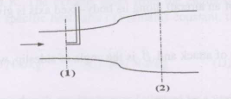
\includegraphics[width=0.5\columnwidth]{figs/36.png}
    \caption{}
    \label{fig:placeholder}
\end{figure}
\hfill(GATE AE 2009)

\begin{multicols}{2}
\begin{enumerate}
\item $-\dfrac{1}{2} \rho \left( 1 - \dfrac{A_1^2}{A_2^2} \right) V_1^2$
\item $\dfrac{1}{2} \rho \left( 1 - \dfrac{A_1^2}{A_2^2} \right) V_1^2$
\item $\dfrac{1}{2} \rho \left( 1 + \dfrac{A_1^2}{A_2^2} \right) V_1^2$
\item $-\dfrac{1}{2} \rho \left( 1 + \dfrac{A_1^2}{A_2^2} \right) V_1^2$
\end{enumerate}
\end{multicols}


\item Two vortices of the same strength and sign are placed a distance $d$ apart as shown below. Assume that the vortices are free to move and the fluid is ideal.

Which of the following statements is true?
\begin{figure}[H]
    \centering
    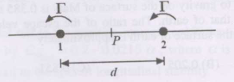
\includegraphics[width=0.5\columnwidth]{figs/37.png}
    \caption{}
    \label{fig:placeholder}
\end{figure}
\hfill(GATE AE 2009)

\begin{enumerate}
\item Vortices 1 and 2 spiral inwards with an initial angular speed $\dfrac{\Gamma}{2 \pi d^2}$ to finally merge and form one vortex of twice the strength.
\item Vortices 1 and 2 spiral inwards with an initial angular speed $\dfrac{\Gamma}{\pi d^2}$ to finally merge and form one vortex of twice the strength.
\item Vortices 1 and 2 perpetually revolve about the midpoint $P$ with radius of revolution $\dfrac{d}{2}$ and angular speed $\dfrac{\Gamma}{2 \pi d^2}$.
\item Vortices 1 and 2 perpetually revolve about the midpoint $P$ with radius of revolution $\dfrac{d}{2}$ and angular speed $\dfrac{\Gamma}{\pi d^2}$.
\end{enumerate}

\item The laminar boundary layer over a large flat plate held parallel to the flow is 7.2 mm thick at a point 0.33 m downstream of the leading edge. If the free stream speed is increased by 50\%, then the new boundary layer thickness at this location will be approximately
\hfill{(GATE AE 2009)}

\begin{multicols}{4}
\begin{enumerate}
\item 10.8 mm
\item 8.8 mm
\item 5.9 mm
\item 4.8 mm
\end{enumerate}
\end{multicols}

\item Consider a simply supported beam of length $2L$ with an overhang of length $L$, loaded by an end moment $M$, as shown below.

\begin{figure}[H]
    \centering
    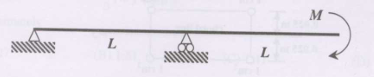
\includegraphics[width=0.5\columnwidth]{figs/39.png}
    \caption{}
    \label{fig:placeholder}
\end{figure}
The bending moment distribution for this beam is

\hfill(GATE AE 2009)

\begin{enumerate}
\item  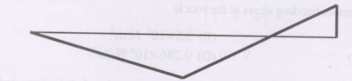
\includegraphics[width=0.5\columnwidth]{figs/A.png}

\item  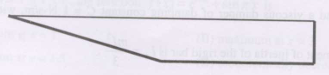
\includegraphics[width=0.5\columnwidth]{figs/B.png}
\item 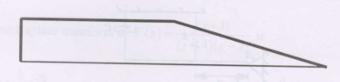
\includegraphics[width=0.5\columnwidth]{figs/C.png}
\item 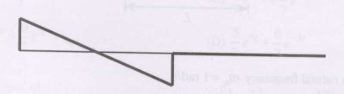
\includegraphics[width=0.5\columnwidth]{figs/D.png}
\end{enumerate}
\item For the spring-mass system shown below, the natural frequencies are

\hfill(GATE AE 2009)
\begin{figure}[H]
    \centering
    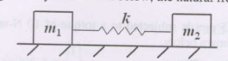
\includegraphics[width=0.5\columnwidth]{figs/40.png}
    \caption{}
    \label{fig:placeholder}
\end{figure}
\begin{enumerate}
\item $0$ and $\sqrt{\dfrac{k(m_1+m_2)}{m_1 m_2}}$
\item $0$ and $\sqrt{\dfrac{k(m_1+m_2)}{2 m_1 m_2}}$
\item $0$ and $\sqrt{\dfrac{k}{m_1+m_2}}$
\item $0$ and $\sqrt{\dfrac{k}{2(m_1+m_2)}}$
\end{enumerate}

\item The buckling load for a simply supported column of rectangular cross section of dimensions $1\,\text{cm} \times 1.5\,\text{cm}$ and length $0.5\,\text{m}$ made of steel $(E = 210 \times 10^9 \text{ N/m}^2)$ is approximately

\hfill(GATE AE 2009)

\begin{enumerate}
\begin{multicols}{4}
    \item 10 kN
\item 4 kN
\item 23 kN
\item 46 kN
\end{multicols}

\end{enumerate}

\item A wing root cross section is idealized using lumped areas (booms) as shown below.

\begin{figure}[H]
    \centering
    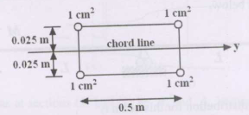
\includegraphics[width=0.5\columnwidth]{figs/42.png}
    \caption{}
    \label{fig:placeholder}
\end{figure}

The wing root bending moment in steady level flight is $M_y = 10$ N-m. If the airplane flies at a load factor $n=3.5$, the maximum bending stress at the root is

\hfill(GATE AE 2009)

\begin{enumerate}
\item $1 \times 10^{6}$ N/m$^{2}$
\item $3.5 \times 10^{6}$ N/m$^{2}$
\item $7 \times 10^{6}$ N/m$^{2}$
\item $0.286 \times 10^{6}$ N/m$^{2}$
\end{enumerate}

\item A uniform rigid bar of mass $m=1$ kg and length $L=1$ m is pivoted at $A$. It is supported by a spring of stiffness $k=1$ N/m and a viscous damper of damping constant $C=1$ N-s/m, with $a=\sqrt{\dfrac{1}{3}}$ m as shown below. The moment of inertia of the rigid bar is $I_A = \dfrac{mL^{2}}{3}$.

\begin{figure}[H]
    \centering
    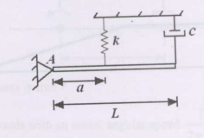
\includegraphics[width=0.5\columnwidth]{figs/43.png}
    \caption{}
    \label{fig:placeholder}
\end{figure}
The system is

\hfill(GATE AE 2009)

\begin{enumerate}
\item overdamped
\item underdamped with natural frequency $\omega_n = 1$ rad/s
\item critically damped
\item underdamped with natural frequency $\omega_n = 2$ rad/s
\end{enumerate}

\item A 2-celled tube with wall thickness 0.5 mm is subjected to a torque of 10 N-m. The resulting shear flows in the two cells are $q_1$ and $q_2$ as shown below.

\begin{figure}[H]
    \centering
    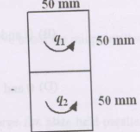
\includegraphics[width=0.35\columnwidth]{figs/44.png}
    \caption{}
    \label{fig:placeholder}
\end{figure}

The torque balance equation (Bredt-Batho formula) for this section leads to

\hfill(GATE AE 2009)

\begin{enumerate}
\begin{multicols}{2}
    \item $q_1 - q_2 = 2000$ N/m
\item $q_1 + 2q_2 = 2000$ N/m
\item $q_1 + q_2 = 2000$ N/m
\item $2q_1 + q_2 = 2000$ N/m
\end{multicols}

\end{enumerate}

\item The value of the integral
\[
\int_0^\pi \frac{dx}{1 + x + \sin x}
\]
evaluated using the trapezoidal rule with two equal intervals is approximately

\hfill(GATE AE 2009)

\begin{enumerate}
\begin{multicols}{4}
 \item 1.27
\item 1.81
\item 1.41
\item 0.71
\end{multicols}

\end{enumerate}

\item The product of the eigenvalues of the matrix
\[
\myvec{
2 & 1 & 1 \\
1 & 3 & 1 \\
1 & 1 & 4
}
\]
is

\hfill(GATE AE 2009)

\begin{enumerate}
\begin{multicols}{4}
\item 20
\item 24
\item 9
\item 17    
\end{multicols}

\end{enumerate}

\item In the interval $1 \leq x \leq 2$, the function $f(x) = e^{x} + \sin \pi x$ is

\hfill(GATE AE 2009)

\begin{enumerate}
\item maximum at $x=1$
\item maximum at $x=2$
\item maximum at $x=1.5$
\item monotonically decreasing
\end{enumerate}

\item The inverse Laplace transform of
\[
F(s) = \frac{s+1}{(s+4)(s-3)}
\]
is

\hfill(GATE AE 2009)

\begin{enumerate}
\item $\dfrac{3}{7} e^{4t} + \dfrac{4}{7} e^{3t}$
\item $\dfrac{3}{7} e^{-4t} + \dfrac{4}{7} e^{3t}$
\item $\dfrac{5}{7} e^{-4t} + \dfrac{6}{7} e^{3t}$
\item $\dfrac{5}{7} e^{4t} + \dfrac{6}{7} e^{-3t}$
\end{enumerate}

\item The linear system of equations $\myvec{A} \mathbf{x} = \mathbf{b}$ where
\[
\myvec{A} = \myvec{1 & 2 \\ 2 & 4}, \quad \mathbf{b} = \myvec{3 \\ 3}
\]
has

\hfill(GATE AE 2009)

\begin{enumerate}
\item no solution
\item infinitely many solutions
\item a unique solution $\mathbf{x} = \myvec{1 \\ 1}$
\item a unique solution $\mathbf{x} = \myvec{0.5 \\ 0.5}$
\end{enumerate}

\item The correct iterative scheme for finding the square root of a positive real number $R$ using the Newton-Raphson method is

\hfill(GATE AE 2009)

\begin{enumerate}
\item $x_{n+1} = \sqrt{R}$
\item $x_{n+1} = \dfrac{1}{2} \left( x_n + \dfrac{R}{x_n} \right)$
\item $x_{n+1} = \dfrac{1}{2} \left( \sqrt{x_n} + \sqrt{\dfrac{R}{x_{n-1}}} \right)$
\item $x_{n+1} = \dfrac{1}{2} \left( \sqrt{R} + x_n \right)$
\end{enumerate}
\textbf{Common Data for Questions 51 and 52:}

The roots of the characteristic equation for the longitudinal dynamics of a certain aircraft are
\[
\lambda_1 = -0.02 + 0.2i, \quad \lambda_2 = -0.02 - 0.2i, \quad \lambda_3 = -2.5 + 2.6i, \quad \lambda_4 = -2.5 - 2.6i,
\]
where \(i = \sqrt{-1}\).

\item The pair of eigenvalues that represent the phugoid mode is

\hfill(GATE AE 2009)

\begin{enumerate}\begin{multicols}{4}
    \item \(\lambda_1\) and \(\lambda_3\)
\item \(\lambda_2\) and \(\lambda_4\)
\item \(\lambda_3\) and \(\lambda_4\)
\item \(\lambda_1\) and \(\lambda_2\)
\end{multicols}

\end{enumerate}

\item The short period damped frequency is

\hfill(GATE AE 2009)

\begin{enumerate}
\begin{multicols}{4}
\item 2.6 rad/s
\item 0.2 rad/s
\item 2.5 rad/s
\item 0.02 rad/s
\end{multicols}

\end{enumerate}

\textbf{Common Data for Questions 53 and 54:}

Consider the vector field \(\myvec{A} \equiv (y^3 + z^3) \myvec{i} + (x^3 + z^3) \myvec{j} + (x^3 + y^3) \myvec{k}\) defined over the unit sphere
\[
x^2 + y^2 + z^2 = 1.
\]

\item The surface integral (taken over the unit sphere) of the component of \(\myvec{A}\) normal to the surface is

\hfill(GATE AE 2009)

\begin{enumerate}
\begin{multicols}{4}
    \item \(\pi\)
\item 1
\item 0
\item \(4 \pi\)
\end{multicols}

\end{enumerate}

\item The magnitude of the component of \(\myvec{A}\) normal to the spherical surface at the point
\[
\myvec{r} = \myvec{\frac{1}{\sqrt{3}}{i} + \frac{1}{\sqrt{3}}{j} + \frac{1}{\sqrt{3}}{k}}
\]
is

\hfill(GATE AE 2009)

\begin{enumerate}
\begin{multicols}{4}
\item \(\frac{1}{3}\)
\item \(\frac{2}{3}\)
\item \(\frac{3}{3}\)
\item \(\frac{4}{3}\)
\end{multicols}

\end{enumerate}
\textbf{Common Data for Questions 55 and 56:}

The partial differential equation for the torsional vibration of a shaft of length \(L\), torsional rigidity \(GJ\), and mass polar moment of inertia per unit length \(I\), is
\[
\frac{\partial^2 \theta}{\partial t^2} = GJ \frac{\partial^2 \theta}{\partial x^2},
\]
where \(\theta\) is the twist.

\item If the shaft is fixed at both ends, the boundary conditions are:

\hfill(GATE AE 2009)

\begin{enumerate}
\item \(\frac{\partial \theta}{\partial x}\bigg|_{x=0} = 0\) and \(\frac{\partial \theta}{\partial x}\bigg|_{x=L} = 0\)
\item \(\theta(0) = 0\) and \(\theta(L) = 0\)
\item \(\frac{\partial \theta}{\partial x}\bigg|_{x=0} = 0\) and \(\theta(L) = 0\)
\item \(\theta(0) = 0\) and \(\frac{\partial \theta}{\partial x}\bigg|_{x=L} = 0\)
\end{enumerate}

\item If the \(n^{\text{th}}\) mode shape of torsional vibration of the above shaft is \(\sin\left( \frac{n \pi x}{L} \right)\), then the \(n^{\text{th}}\) natural frequency of vibration, i.e., \(\omega_n\), is given by

\hfill(GATE AE 2009)

\begin{enumerate}
\item \(\omega_n = \frac{n \pi}{L} \sqrt{\frac{GJ}{I}}\)
\item \(\omega_n = \frac{(2n+1)\pi}{2L} \sqrt{\frac{GJ}{I}}\)
\item \(\omega_n = \frac{n \pi}{2L} \sqrt{\frac{GJ}{I}}\)
\item \(\omega_n = \frac{(2n+1)\pi}{L} \sqrt{\frac{GJ}{I}}\)
\end{enumerate}

\textbf{Statement for Linked Answer Questions 57 and 58:}

Air enters the combustor of a gas-turbine engine at a total temperature \(T_0\) of 500 K. The air stream is split into two parts: primary and secondary streams. The primary stream reacts with fuel supplied at a fuel-air ratio of 0.05. The resulting combustion products are then mixed with the secondary air stream to obtain gas with total temperature of 1550 K at the turbine inlet. The fuel has a heating value of 42 MJ/kg. The specific heats of air and combustion products are taken as \(c_p = 1\ \mathrm{kJ/kg/K}\).

\item If the sensible enthalpy of fuel is neglected, the temperature of combustion products from the reaction of primary air stream with fuel is approximately

\hfill(GATE AE 2009)

\begin{enumerate}
\item 2100 K
\item 3200 K
\item 2600 K
\item 1800 K
\end{enumerate}

\item The approximate ratio of mass flow rates of the primary air stream to the secondary air stream required to achieve the turbine inlet total temperature of 1550 K is

\hfill(GATE AE 2009)

\begin{enumerate}
\item 2:1
\item 1:2
\item 1:1.5
\item 1:1
\end{enumerate}

\textbf{Statement for Linked Answer Questions 59 and 60:}

A piston compresses 1 kg of air inside a cylinder as shown

\begin{figure}[H]
    \centering
    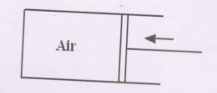
\includegraphics[width=0.5\columnwidth]{figs/img.png}
    \caption{}
    \label{fig:placeholder}
\end{figure}
The rate at which the piston does work on the air is 3000 W. At the same time, heat is being lost through the walls of the cylinder at a rate of 847.5 W.

\item After 10 seconds, the change in specific internal energy of the air is

\hfill(GATE AE 2009)

\begin{enumerate}
\item 21,525 J/kg
\item -21,525 J/kg
\item 30,000 J/kg
\item -8,475 J/kg
\end{enumerate}

\item Given that the specific heats of air at constant pressure and volume are \(c_p = 1004.5\ \mathrm{J/kg{\cdot}K}\) and \(c_v = 717.5\ \mathrm{J/kg{\cdot}K}\) respectively, the corresponding change in the temperature of the air is

\hfill(GATE AE 2009)

\begin{enumerate}
\item 21.4 K
\item -21.4 K
\item 30 K
\item -30 K
\end{enumerate}



\begin{center}
    \textbf{END OF THE QUESTION PAPER}
\end{center}

\end{enumerate}
\end{flushleft}
\end{document}


